\chapter{Anoushabour}
\label{ch:anoushabour}
\index{dessert}
\index{pudding}

\marginnote{
    \textbf{Makes 1 bowl} \\
    Prep time: 30 minutes + overnight rest \\
    Cook time: 45 minutes \\
    \vspace*{\baselineskip}

    1 cup pearl barley \\
    1/4 cup sugar \\
    Yellow and sultan raisins \\
    Dried apricots, quartered \\
    1/4 tsp rose water or orange blossom water, optional 
}

% \begin{figure}
%   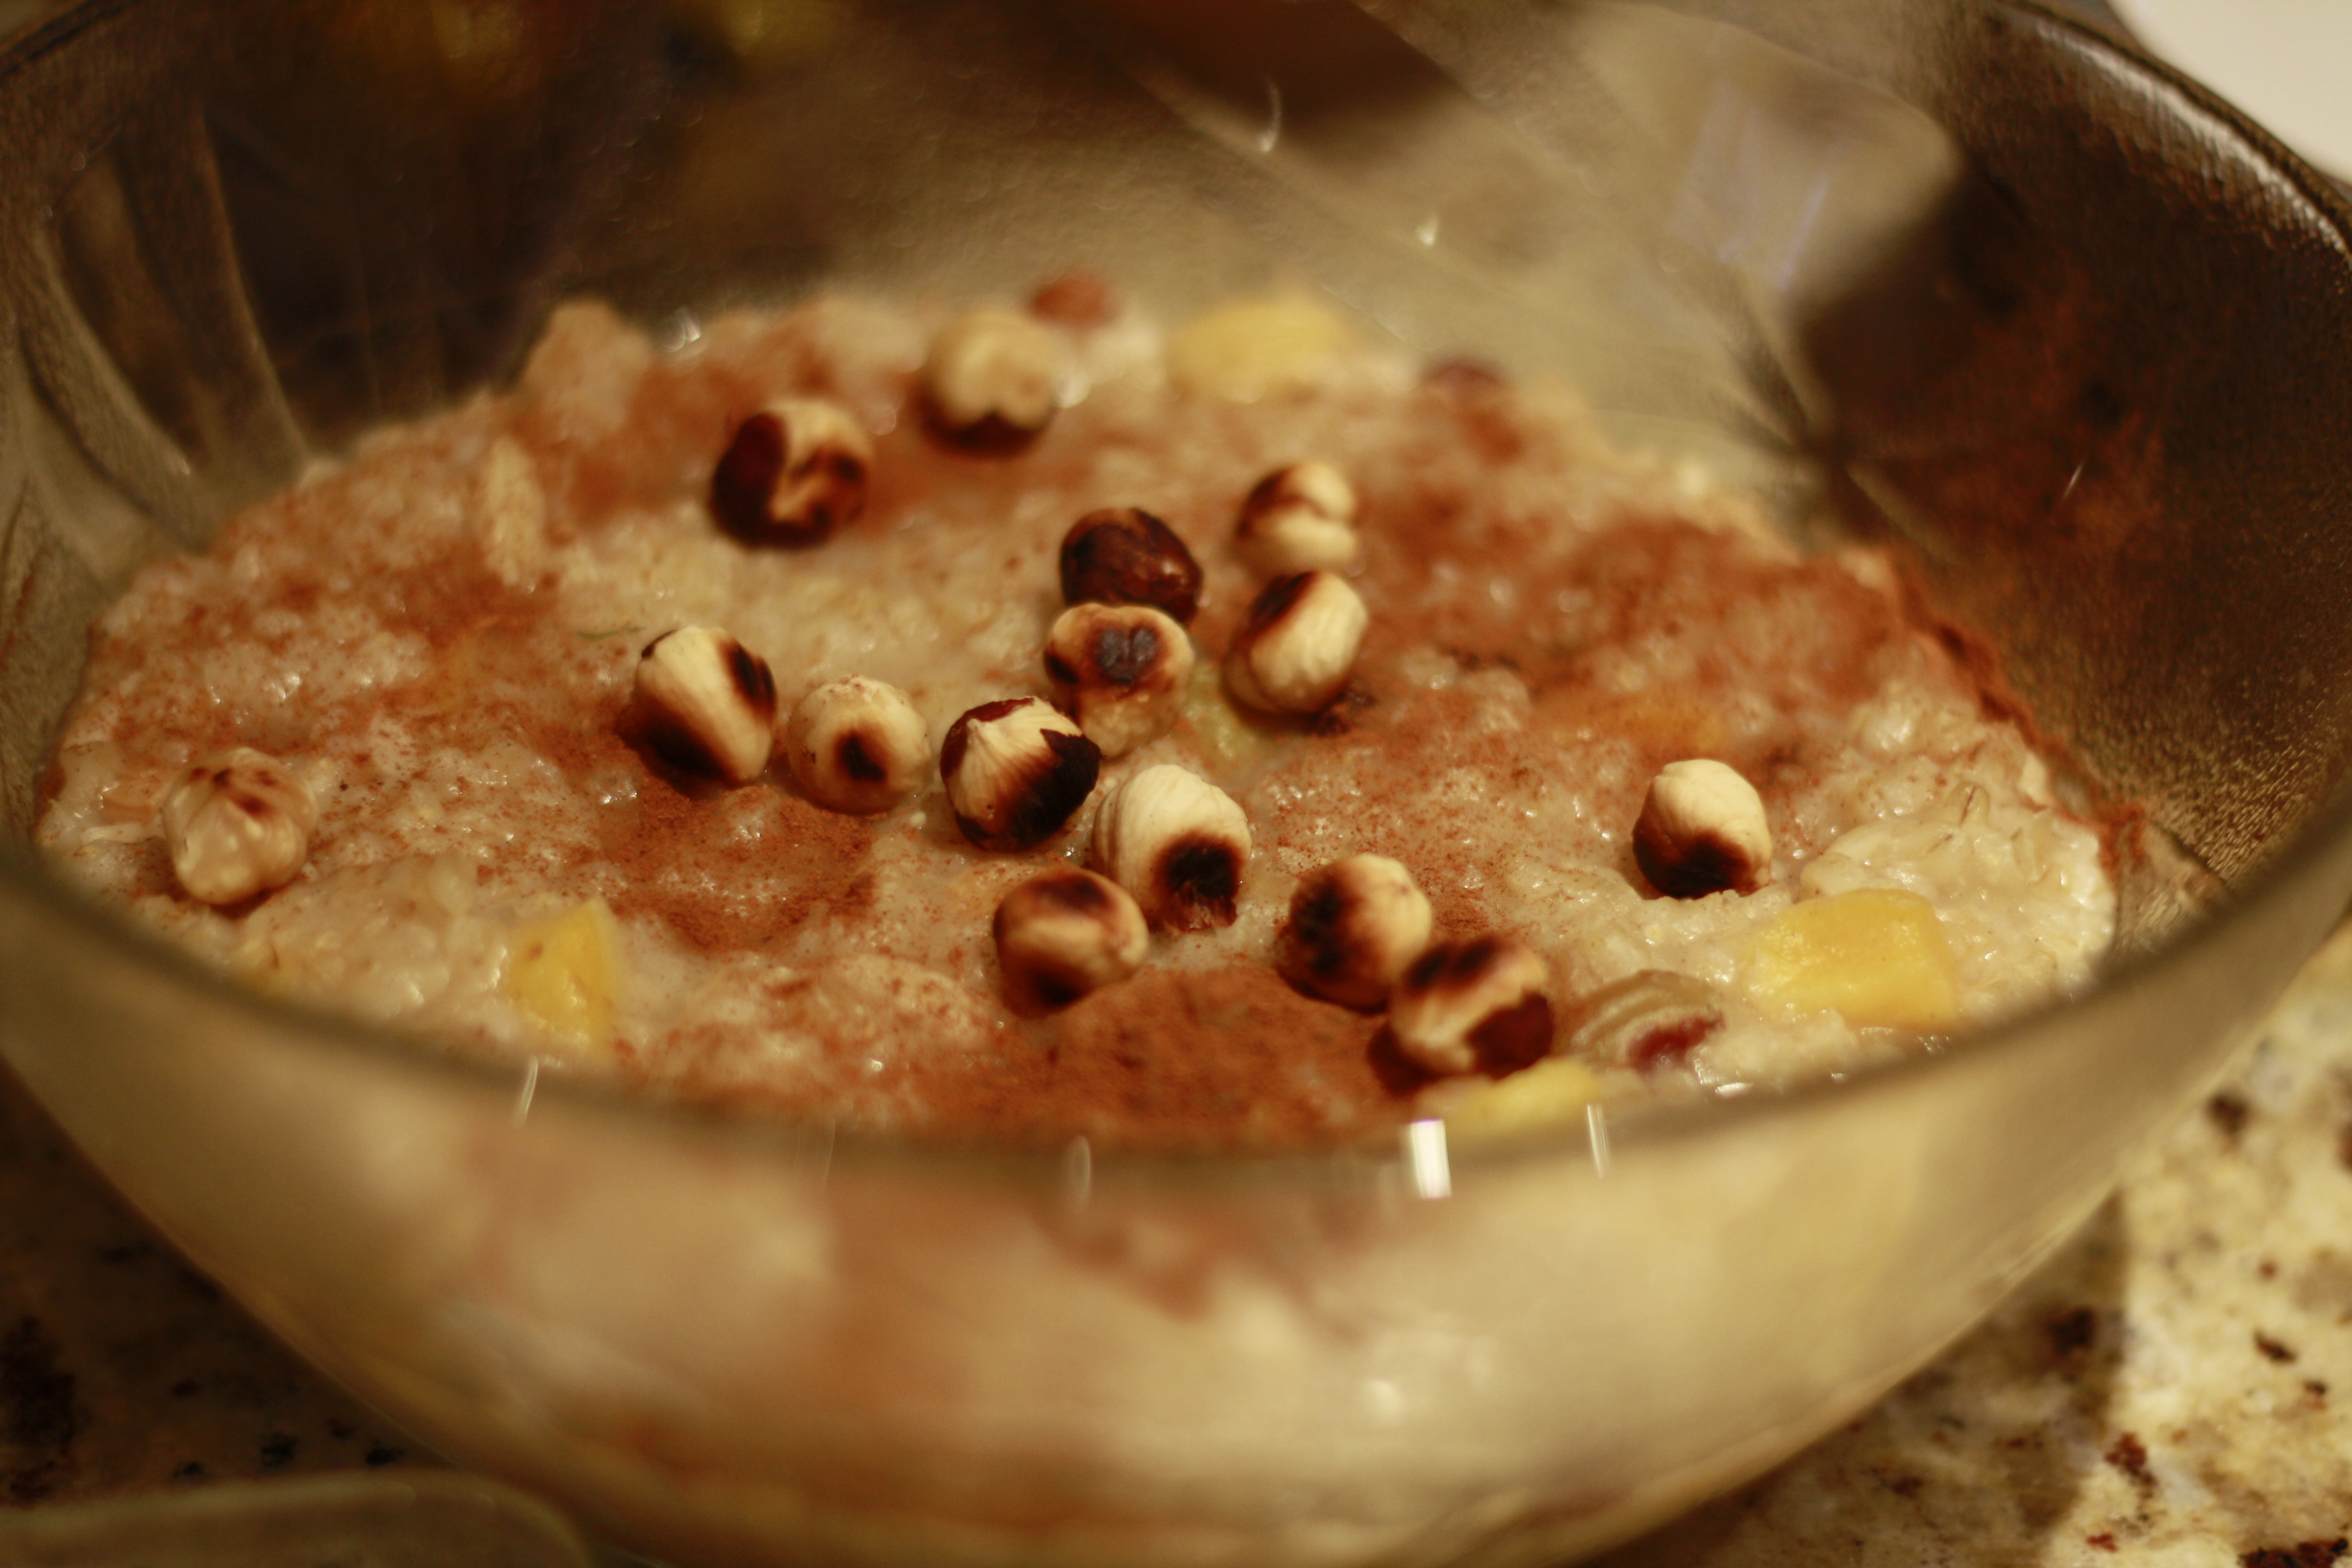
\includegraphics[width=60mm]{dermardiros/images/Anoushabour.JPG}
%     \caption{Anoushabour from New Year's Eve brunch at AJ and Eddy's in 2011!}
% \end{figure}
\marginalfigure{dermardiros/images/Anoushabour.JPG}{Anoushabour from New Year's Eve brunch at AJ and Eddy's in 2011!}{fig:anoushabour}

\textit{Sweet barley pudding}

Family member: Sybil

\begin{enumerate}
    \item In a pot, cook pearl barley in 2 cups of water for 10 minutes.
    \item Remove from stove, let cool. Cover and leave overnight.
    \item The next day, the barley should be plump. Add a little more water, the raisins and apricots. Continue to cook for a few minutes. There should be water in the pot (not completely absorbed).
    \item After 15 minutes, add the sugar and continue cooking for 15 minutes more.
    \item Once done, remove from heat, add rose water or orange blossom water if using, and let it cool.
    \item Pour in a large glass bowl and serve.
\end{enumerate}
